% ============================================================================
%  MINIMAX-OPTIMALITY OF THE ADAPT/FREEZE/ABSTAIN CERTIFICATE
%  ON THE IDENTIFIABLE SIDE OF THE BENEFIT-SIGN FRONTIER  (theory_v2, Wave 2)
%
%  Target: a matching minimax LOWER bound on the sample complexity to certify
%  sign(Delta) at false-adapt <= alpha over ALL valid label-free rules, pairing
%  with the certificate's upper bound (thm:cert).  RESULT: ORDER-OPTIMAL
%  (matched rate n ASYMP (sigma^2/Delta^2) log(1/alpha); leading-constant ratio
%  -> 4 as alpha -> 0).  Tight constants are NOT claimed (a separate open problem).
%
%  Macros required (already in kbound.tex / main_theory_5.tex):
%    \E \Pr \sign \TV \Law \R ; theorem/lemma/proposition/corollary/remark envs;
%    \textsc{adapt}/\textsc{freeze}/\textsc{abstain}.
%  External refs used: thm:cert, thm:imp, thm:frontier, prop:lecam-finite,
%    thm:rate-ub, thm:rate-lb (the last two from knowability_rates.tex).
%  Validator: theory_v2/val_minimax_optimality.py
%             -> minimax_optimality_results.json ; fig_minimax_optimality.png.
% ============================================================================
\providecommand{\TV}{\mathrm{TV}}
\providecommand{\KL}{\mathrm{KL}}
\section{Minimax-optimality of the certificate on the identifiable side}\label{sec:minimax-opt}

The certificate of Theorem~\ref{thm:cert} commits \textsc{adapt}/\textsc{freeze} only
outside an abstain band and is \emph{valid} --- its marginal false-adapt and false-freeze
rates are each $\le\alpha$. Validity alone does not preclude a competitor that certifies the
same decision from fewer samples. This section settles, on the \emph{identifiable} side of the
frontier ($|M|>\beta$, Theorem~\ref{thm:frontier}), whether the certificate's
\emph{sample complexity} is best possible among \emph{all} valid label-free rules. The answer
is \emph{order-optimal}: a Le~Cam two-point lower bound matches the certificate's upper bound up
to universal constants. We are explicit about scope: the minimax object is the
\emph{two-sided committal error of a label-free decision rule}, the class is a Gaussian (and,
for robustness, a bounded) location family on the identifiable side, and we prove
\emph{order}-optimality (rate $+$ bounded constant ratio), not tight constants.

\subsection{The minimax sample complexity, and the decision class}

\begin{definition}[Two-sided certifying rule and its sample complexity]\label{def:certifying}
Fix a noise scale $\sigma>0$, a margin $\Delta>0$, and a level $\alpha\in(0,\tfrac14)$.
Let $\mathcal P^n_{\Delta,\sigma}=\{P^n_{+},P^n_{-}\}$ be the two \emph{identifiable-side} worlds
in which $n$ i.i.d.\ paired benefits $X_1,\dots,X_n$ are observed with
$\E[X_i]=+\Delta$ (world $P_+$, so $\sign\Delta=+$, \textsc{adapt} is the Bayes action) and
$\E[X_i]=-\Delta$ (world $P_-$, so \textsc{freeze} is Bayes), respectively, both with
per-sample variance proxy $\le\sigma^2$. A (possibly randomized) \emph{label-free decision rule}
is a measurable map $g:(X_1,\dots,X_n)\mapsto\{\textsc{adapt},\textsc{freeze},\textsc{abstain}\}$.
Its committal-error and miss probabilities are
\[
  \mathrm{FA}(g)=\Pr_{P_-}\!\big(g=\textsc{adapt}\big),\quad
  \mathrm{FF}(g)=\Pr_{P_+}\!\big(g=\textsc{freeze}\big),\quad
  \mathrm{miss}_+(g)=\Pr_{P_+}\!\big(g\neq\textsc{adapt}\big),\quad
  \mathrm{miss}_-(g)=\Pr_{P_-}\!\big(g\neq\textsc{freeze}\big).
\]
Here $\mathrm{FA},\mathrm{FF}$ are \emph{wrong-commit} (false-adapt / false-freeze) rates and
$\mathrm{miss}_\pm$ are \emph{failure-to-certify} (the correct action is not committed --- it is
either abstained or, worse, reversed). Call $g$ \emph{$\alpha$-certifying} if it meets the same
two-sided guarantee the certificate provides:
\[
   \mathrm{FA}(g)\le\alpha,\quad \mathrm{FF}(g)\le\alpha,\quad
   \mathrm{miss}_+(g)\le\alpha,\quad \mathrm{miss}_-(g)\le\alpha .
\]
Equivalently, in each world $g$ commits to the \emph{correct} action with probability $\ge1-\alpha$
and to the \emph{wrong} action with probability $\le\alpha$ (the miss bound subsumes the
wrong-commit bound, since a wrong commit is a special miss). The \emph{minimax certifying sample
complexity} is
\[
  n^\star(\Delta,\sigma,\alpha)
  \;=\;\min\big\{\,n\in\mathbb N:\ \exists\ \text{an $\alpha$-certifying label-free rule on }
  \mathcal P^n_{\Delta,\sigma}\big\}.
\]
\end{definition}

\begin{remark}[Why the miss bound, and why it is the right comparison class]\label{rmk:miss-bound}
The guarantee ``$\mathrm{miss}_\pm\le\alpha$ and $\mathrm{FA},\mathrm{FF}\le\alpha$'' is precisely
what Theorem~\ref{thm:cert} delivers on the identifiable side: once the radius
$\varepsilon_n<\Delta$, the certificate commits to the correct sign with probability $\ge1-\alpha$
(so $\mathrm{miss}\le\alpha$) and never wrong-commits beyond the calibration's $\alpha$-event. The
minimax statement is therefore a comparison among \emph{all label-free rules that achieve the
certificate's own two-sided $\alpha$-guarantee}: we ask whether any of them needs fewer samples.
This is the honest and decision-relevant comparison; relaxing the miss bound to ``commit correctly
with probability $\ge\tfrac12$'' (mere consistency) weakens the lower bound to a \emph{constant}
(no $\log(1/\alpha)$), recovering only the floor of Theorem~\ref{thm:imp} ---
see Remark~\ref{rmk:opt-delicate}. The $\log(1/\alpha)$ rate is exactly the cost of the small
\emph{miss} (power-side) error, and it binds any rule that wants the certificate's confidence.
\end{remark}

\noindent The pair $\{P_+,P_-\}$ lies strictly on the identifiable side: with the frontier
parametrization of Theorem~\ref{thm:frontier} one may take $\gamma=0$, so the observable margin
is $|M|=\Delta>\beta=0$ and $\sign\Delta=\sign M$ is point-identified. Thus
Definition~\ref{def:certifying} measures, on the \emph{knowable} part of the problem, the
information cost of \emph{statistically} certifying a sign that is \emph{population}-identified.
This is the complement of the impossibility regime of Theorem~\ref{thm:imp} (where $\TV=0$ and no
$n$ suffices) and of the constant-floor regime of Proposition~\ref{prop:lecam-finite} (where the
two worlds are rescaled to stay equally hard as $n\to\infty$); here the worlds are
\emph{fixed} and we ask how fast certification becomes possible.

\subsection{The matching bounds}

\begin{theorem}[Order-optimal sample complexity to certify the benefit sign]\label{thm:minimax-opt}
For every $\sigma>0$, $\Delta>0$, and $\alpha\in(0,\tfrac14)$, the minimax certifying sample
complexity of Definition~\ref{def:certifying} obeys
\[
   \boxed{\;
   \frac{\sigma^2}{2\Delta^2}\,\log\!\frac{1}{4\alpha}
   \;\le\;
   n^\star(\Delta,\sigma,\alpha)
   \;\le\;
   \frac{2\sigma^2}{\Delta^2}\,\log\!\frac{2}{\alpha}\;+\;1 .
   \;}
\]
Consequently
\[
   n^\star(\Delta,\sigma,\alpha)\;\asymp\;\frac{\sigma^2}{\Delta^2}\,\log\frac1\alpha ,
\]
and the deployed empirical-Bernstein certificate of Theorem~\ref{thm:cert}
attains this rate: it is \emph{minimax order-optimal} on the identifiable side, with the ratio
of the upper to the lower leading constant tending to $4$ as $\alpha\to0$. The lower bound holds
over the Gaussian location family $X_i\sim\mathcal N(\pm\Delta,\sigma^2)$ and, with the
constant degraded only by an absolute factor, over the bounded family
$X_i\in\{-1,+1\}$ with $\E X_i=\pm\Delta$ (variance proxy $\sigma^2=1-\Delta^2$).
\end{theorem}

\begin{remark}[What is and is not claimed]\label{rmk:opt-scope}
(i) The risk bounded is the \emph{two-sided committal error} of a label-free \emph{decision}
rule, not estimation risk; the certified estimand is $\sign\Delta$, on the identifiable side
$|M|>\beta$. (ii) The match is to \emph{order} (rate $\sigma^2/\Delta^2$ \emph{and} dependence
$\log(1/\alpha)$, with a bounded constant ratio), not to a tight constant; closing the residual
factor (here $\to4$) is the separately-listed tight-constants open problem
(\S\ref{sec:consolidation}; \texttt{knowability\_rates.tex}, \texttt{onebit\_audit\_rate.tex}).
(iii) The lower bound is information-theoretic: it binds \emph{every} $\alpha$-valid label-free
rule with nontrivial power, certificate or not. (iv) The $\log(1/\alpha)$ factor is genuinely a
\emph{two-sided} effect: it appears precisely because both error probabilities are constrained
to be $\le\alpha$. A one-sided two-point bound (as in Theorem~\ref{thm:imp} and
Proposition~\ref{prop:lecam-finite}, which constrain a single mixed error) yields the rate
$\sigma^2/\Delta^2$ \emph{without} the logarithm; the logarithm is the price of small
\emph{power-side} error, in exact analogy with the Chernoff--Stein lemma.
\end{remark}

\subsection{Proof}

The two directions are independent. The upper bound is a restatement of the deployed
certificate; the lower bound is Le~Cam's two-point method at the decision boundary, finished by
Bretagnolle--Huber. We first record the standard tools.

\begin{lemma}[Le Cam two-point inequality for the two-sided error]\label{lem:lecam-twosided}
Let $Q_0,Q_1$ be two laws on a common space and let $\psi$ be any (randomized) test
$\psi:\,\cdot\mapsto\{0,1\}$. Write the two error probabilities
$e_0(\psi)=Q_0(\psi=1)$ and $e_1(\psi)=Q_1(\psi=0)$. Then
\[
   e_0(\psi)+e_1(\psi)\;\ge\;1-\TV(Q_0,Q_1)\;\ge\;\tfrac12\exp\!\big(-\mathrm{KL}(Q_0\,\|\,Q_1)\big).
\]
The first inequality is Le~Cam's testing-affinity bound \cite{lecam1986asymptotic};
the second is the Bretagnolle--Huber inequality
$1-\TV(Q_0,Q_1)\ge\tfrac12 e^{-\mathrm{KL}(Q_0\|Q_1)}$.
\end{lemma}

\begin{proof}
For the first inequality, $e_0(\psi)+e_1(\psi)=Q_0(\psi=1)+Q_1(\psi=0)\ge
\inf_{A}\big(Q_0(A)+Q_1(A^c)\big)=1-\TV(Q_0,Q_1)$, the infimum over events $A$ attained by the
likelihood-ratio test and equal to the testing affinity. The second inequality is
Bretagnolle--Huber \cite[Ch.~2, Lemma~2.6]{tsybakov2009introduction}; see also the elementary proof via
$\TV\le\sqrt{1-e^{-\mathrm{KL}}}$, which rearranges to $1-\TV\ge1-\sqrt{1-e^{-\mathrm{KL}}}\ge
\tfrac12 e^{-\mathrm{KL}}$ (the last step since $1-\sqrt{1-u}\ge u/2$ for $u\in[0,1]$, with
$u=e^{-\mathrm{KL}}$).
\end{proof}

\begin{lemma}[Gaussian two-point KL]\label{lem:gauss-kl}
For the product Gaussians $P^n_{+}=\mathcal N(+\Delta,\sigma^2)^{\otimes n}$ and
$P^n_{-}=\mathcal N(-\Delta,\sigma^2)^{\otimes n}$,
\[
   \mathrm{KL}\big(P^n_{+}\,\|\,P^n_{-}\big)
   \;=\;n\cdot\frac{(2\Delta)^2}{2\sigma^2}
   \;=\;\frac{2n\Delta^2}{\sigma^2}.
\]
\end{lemma}
\begin{proof}
Per coordinate, $\mathrm{KL}(\mathcal N(\mu_1,\sigma^2)\|\mathcal N(\mu_2,\sigma^2))=
(\mu_1-\mu_2)^2/(2\sigma^2)$; here $\mu_1-\mu_2=2\Delta$. KL tensorizes over independent
coordinates, giving the stated $n$-fold value.
\end{proof}

\paragraph{Upper bound (achievability; the certificate).}
This is Theorem~\ref{thm:cert} instantiated on $\mathcal P^n_{\Delta,\sigma}$. Run the certificate
with $\hat\Delta=\bar X_n=\tfrac1n\sum_i X_i$ and a sub-Gaussian/empirical-Bernstein radius
$\varepsilon_n(\alpha)$ valid at level $\alpha$, deciding \textsc{adapt} if
$\bar X_n-\varepsilon_n>0$, \textsc{freeze} if $\bar X_n+\varepsilon_n<0$, else \textsc{abstain}.
Validity (the false-adapt and false-freeze rates are each $\le\alpha$ in \emph{every} world,
hence in $P_\mp$) is exactly the marginal guarantee of Theorem~\ref{thm:cert}: on the
$(1-\alpha)$ event $\{|\bar X_n-\Delta|\le\varepsilon_n\}$, committing \textsc{adapt} forces
$\Delta\ge\bar X_n-\varepsilon_n>0$, so a wrong commit lives in the complementary $\alpha$-event.
For the certifying (power) side, the leading (variance) term of the radius is
$\varepsilon_n(\alpha)=\sigma\sqrt{2\log(2/\alpha)/n}\,(1+o(1))$
(sub-Gaussian concentration; the Maurer--Pontil empirical-Bernstein radius of
Proposition~\ref{thm:rate-ub} self-normalizes to the same leading term and adds only a
lower-order $O\!\big(R\log(1/\alpha)/n\big)$ range term). Whenever
$\varepsilon_n(\alpha)<\Delta$, i.e.\
\[
   \sigma\sqrt{\tfrac{2\log(2/\alpha)}{n}}<\Delta
   \quad\Longleftrightarrow\quad
   n>\frac{2\sigma^2}{\Delta^2}\log\frac2\alpha ,
\]
the event $\{|\bar X_n-\Delta|\le\varepsilon_n\}$ (probability $\ge1-\alpha\ge\tfrac12$) is
contained in $\{\bar X_n-\varepsilon_n>0\}$ in world $P_+$, so the correct action is committed
with probability $\ge1-\alpha\ge\tfrac12$; world $P_-$ is symmetric. Hence the certificate is
$\alpha$-certifying once $n>\tfrac{2\sigma^2}{\Delta^2}\log(2/\alpha)$, which gives
$n^\star\le\tfrac{2\sigma^2}{\Delta^2}\log(2/\alpha)+1$. (The bounded-benefit version is
identical with $\sigma^2=1-\Delta^2$ and the extra $O(R/\Delta)$ range term, which is
lower-order in the regime $\sigma/\Delta\gg1$.) \hfill$\square$

\paragraph{Lower bound (the two-point obstruction).}
Suppose some label-free rule $g$ is $\alpha$-certifying on $\mathcal P^n_{\Delta,\sigma}$. Collapse
$g$ to the single binary test $\psi=\mathbf 1[g=\textsc{adapt}]$, viewed as a test of the null
$Q_0:=P^n_{-}$ against the alternative $Q_1:=P^n_{+}$. Its two error probabilities are
\emph{exactly} two of the rule's certifying quantities:
\[
   e_0(\psi)=\Pr_{P_-}(\psi=1)=\Pr_{P_-}(g=\textsc{adapt})=\mathrm{FA}(g)\ \le\ \alpha,
\]
\[
   e_1(\psi)=\Pr_{P_+}(\psi=0)=\Pr_{P_+}(g\neq\textsc{adapt})=\mathrm{miss}_+(g)\ \le\ \alpha .
\]
The second line is the crux and is where the miss bound of Definition~\ref{def:certifying} is
used: because $g$ certifies, it commits to \textsc{adapt} in world $P_+$ with probability
$\ge1-\alpha$, so the event $\{g\neq\textsc{adapt}\}$ (abstain \emph{or} freeze) has probability
$\le\alpha$. Thus $\psi$ is a single test with \emph{both} error probabilities $\le\alpha$ --- no
symmetrization, coin-flipping, or power-vs-TV detour is needed; abstention is simply counted as a
miss, which the certifying assumption already controls. Lemma~\ref{lem:lecam-twosided} (with the
Bretagnolle--Huber branch) and Lemma~\ref{lem:gauss-kl} then give
\[
   2\alpha\ \ge\ e_0(\psi)+e_1(\psi)\ \ge\ \tfrac12\exp\!\big(-\mathrm{KL}(P^n_-\|P^n_+)\big)
   \ =\ \tfrac12\exp\!\Big(-\tfrac{2n\Delta^2}{\sigma^2}\Big).
\tag{$\ast$}
\]
(We used $\mathrm{KL}(P^n_-\|P^n_+)=\mathrm{KL}(P^n_+\|P^n_-)=2n\Delta^2/\sigma^2$ by
symmetry.) Solving ($\ast$) for $n$,
\[
   \exp\!\Big(-\tfrac{2n\Delta^2}{\sigma^2}\Big)\le 4\alpha
   \quad\Longleftrightarrow\quad
   \frac{2n\Delta^2}{\sigma^2}\ \ge\ \log\frac1{4\alpha}
   \quad\Longleftrightarrow\quad
   n\ \ge\ \frac{\sigma^2}{2\Delta^2}\,\log\frac1{4\alpha}.
\]
Therefore \emph{every} $\alpha$-certifying label-free rule requires
$n\ge\tfrac{\sigma^2}{2\Delta^2}\log\frac1{4\alpha}$, i.e.\
$n^\star(\Delta,\sigma,\alpha)\ge\tfrac{\sigma^2}{2\Delta^2}\log\frac1{4\alpha}$ (the bound is
vacuous, and nothing is claimed, once $\alpha\ge\tfrac14$, which is why $\alpha<\tfrac14$ is
assumed). The bounded-family claim follows verbatim with $\mathrm{KL}$ of two $\{-1,+1\}$ Bernoulli
laws with means $\pm\Delta$ in place of Lemma~\ref{lem:gauss-kl}: that per-sample KL equals
$\tfrac{1+\Delta}{2}\log\tfrac{1+\Delta}{1-\Delta}+\tfrac{1-\Delta}{2}\log\tfrac{1-\Delta}{1+\Delta}
=2\Delta\,\mathrm{artanh}\,\Delta=\tfrac{2\Delta^2}{1-\Delta^2}+O(\Delta^4)$, so with the bounded
variance proxy $\sigma^2=1-\Delta^2$ the same $n\gtrsim(\sigma^2/\Delta^2)\log(1/\alpha)$ bound
holds up to the absolute constant. \hfill$\square$

\medskip
\noindent Combining the two displays yields the boxed sandwich, and the ratio of leading
constants is $\big(\tfrac{2\sigma^2}{\Delta^2}\log\tfrac2\alpha\big)\big/\big(\tfrac{\sigma^2}{2
\Delta^2}\log\tfrac1{4\alpha}\big)=4\cdot\log(2/\alpha)/\log(1/(4\alpha))\to4$ as $\alpha\to0$.
This proves Theorem~\ref{thm:minimax-opt}.\qed

\begin{remark}[Where the proof is delicate, and the honest gap]\label{rmk:opt-delicate}
The single subtle point is the three-way-to-two-way reduction: a rule may \emph{abstain}, so
$\psi=\mathbf 1[g=\textsc{adapt}]$ is a genuine binary test only after one decides how to score
abstention. The reduction succeeds because abstention is counted as a \emph{miss} in world $P_+$:
the certifying requirement $\mathrm{miss}_+(g)\le\alpha$ bounds
$e_1(\psi)=\Pr_{P_+}(g\neq\textsc{adapt})$ \emph{directly}, with no power-vs-affinity detour and
no symmetrization --- the type-II error of $\psi$ \emph{is} $\mathrm{miss}_+(g)$ by definition.
This is the entire role of the miss bound in Definition~\ref{def:certifying}, and it is what makes
($\ast$) a clean two-sided $\{\alpha,\alpha\}$ test to which Bretagnolle--Huber applies, producing
the $\log(1/(4\alpha))$ factor. The dependence of the bound on the \emph{strength} of the
power-side requirement is real and is the honest soft spot of the statement: if ``certifying'' is
weakened from $\mathrm{miss}_+\le\alpha$ to mere consistency (correct-commit $\ge\tfrac12$, i.e.\
$e_1\le\tfrac12$), then ($\ast$) becomes $\alpha+\tfrac12\ge\tfrac12 e^{-\mathrm{KL}}$, whose
solution $n\ge\tfrac{\sigma^2}{2\Delta^2}\log\tfrac1{1+2\alpha}$ carries \emph{no}
$\log(1/\alpha)$ --- it collapses to the constant floor of Theorem~\ref{thm:imp}. Thus the
$\log(1/\alpha)$ rate is \emph{exactly} the price of the small power-side ($\mathrm{miss}$) error
and binds only rules that demand the certificate's two-sided confidence; against the weaker
consistency benchmark the certificate is \emph{not} claimed order-optimal in $\alpha$. The
factor-$4$ gap between the boxed leading constants is likewise genuine and not claimed tight
(Remark~\ref{rmk:opt-scope}(ii)): it is the known looseness of Bretagnolle--Huber against the
exact Gaussian frontier $n_{\mathrm{opt}}=(\sigma/\Delta)^2 z_{1-\alpha}^2$, which the validator
confirms satisfies $n_{\mathrm{LB}}\le n_{\mathrm{opt}}\le n_{\mathrm{UB}}$ with
$n_{\mathrm{opt}}/n_{\mathrm{LB}}\approx3.3$--$3.6$ throughout (so the lower bound never exceeds
the true frontier --- the bound is sound, not optimistic).
\end{remark}

\subsection{Relation to the existing rate propositions}

Theorem~\ref{thm:minimax-opt} is the \emph{decision-theoretic} counterpart of the
margin-rate propositions of \texttt{knowability\_rates.tex}
(Propositions~\ref{thm:rate-ub}--\ref{thm:rate-lb}). Those bound the smallest
\emph{$(\alpha,\beta)$-reliable margin} $\kappa_n$ as a function of $n$; inverting
$\kappa_n\asymp\sigma\sqrt{\log(1/\bar\alpha)/n}$ for a fixed margin $\Delta$ recovers exactly the
sample-complexity statement here. The present formulation makes three things explicit that the
margin form leaves implicit: (i) the minimax object is the two-sided committal error of a
\emph{decision} rule on the identifiable side, not a margin; (ii) the $\log(1/\alpha)$ factor is a
\emph{two-sided} (power-side) effect, distinguishing it cleanly from the one-sided constant floor
of Theorem~\ref{thm:imp} and Proposition~\ref{prop:lecam-finite}, which carry \emph{no}
logarithm; and (iii) the certificate \emph{already deployed} is the achiever, so optimality is a
property of the shipped rule, adaptively in $\sigma$ (Proposition~\ref{thm:rate-ub}). The dense
branch of Proposition~\ref{thm:rate-lb} and the bound here are the same Bretagnolle--Huber
two-point estimate viewed through margin vs.\ sample-size duality.

\begin{corollary}[Minimax order-optimality of the certificate]\label{cor:cert-minimax}
On the identifiable side $|M|>\beta$ of the benefit-sign frontier
(Theorem~\ref{thm:frontier}), the adapt/freeze/abstain certificate of Theorem~\ref{thm:cert} is
minimax order-optimal for certifying $\sign\Delta$ at two-sided level $\alpha$: its sample
complexity $\tfrac{2\sigma^2}{\Delta^2}\log(2/\alpha)+O(R/\Delta\cdot\log(1/\alpha))$ matches the
information-theoretic floor $\tfrac{\sigma^2}{2\Delta^2}\log\tfrac1{4\alpha}$ over all
$\alpha$-valid label-free rules, up to a universal constant ($\to4$ on the leading term). No
valid label-free procedure --- certificate or otherwise --- certifies the sign from
asymptotically fewer samples.
\end{corollary}

\paragraph{Numerical validation.}
\texttt{theory\_v2/val\_minimax\_optimality.py} (seeds fixed; \texttt{numpy}; runs in
$<\!40$\,s) certifies all components against
\texttt{minimax\_optimality\_results.json} and Fig.~\ref{fig:minimax-opt}:
\textbf{[A]} the Bretagnolle--Huber bound $\tfrac12 e^{-\mathrm{KL}}$ lower-bounds the
\emph{exact} optimal mixed error $\Phi(-\sqrt n\,\Delta/\sigma)$ at every tested
$(\Delta,\sigma,n)$, and the analytic optimum matches Monte-Carlo to $<\!5\times10^{-3}$;
\textbf{[B]} the exact frontier $n_{\mathrm{opt}}=(\sigma/\Delta)^2 z_{1-\alpha}^2$ satisfies the
sandwich $n_{\mathrm{LB}}\le n_{\mathrm{opt}}\le n_{\mathrm{UB}}$ for every $(\Delta,\alpha)$, has
log--log slope $2.00$ in $1/\Delta$ (theory $2$), and $n_{\mathrm{opt}}/n_{\mathrm{LB}}$ is a
universal constant $\approx 3.3$--$3.5$ for $\alpha\le0.1$; the upper/lower leading-constant ratio
$\to4$;
\textbf{[C]} the deployed empirical-Bernstein certificate keeps false-adapt $\le\alpha$ at
\emph{every} $n$ (validity), and its empirical certifying-$n$ grows linearly in $\log(1/\alpha)$
at the upper-bound slope and as $1/\Delta^2$ (log--log slope $2.14$), i.e.\ at the predicted rate;
\textbf{[D]} a brute-force panel of label-free rules (sign-thresholds and polarities on the
sample mean, median, $20\%$-trimmed mean, sign-count, and clipped mean) finds \emph{no} rule with
both wrong-commit rates $\le\alpha$ \emph{and} nontrivial power (correct-commit $\ge\tfrac12$) at
$n<n_{\mathrm{LB}}$, while such a rule does exist at and above $n_{\mathrm{LB}}$ --- the two-point
obstruction is real, not an artifact of the certificate's conservativeness. (We probe the
power-relaxed certifying set here, matching the lower-bound construction; \emph{full}
$\alpha$-certification requires the larger $n_{\mathrm{opt}}=(\sigma/\Delta)^2z_{1-\alpha}^2$,
which $n_{\mathrm{LB}}$ correctly lower-bounds, $n_{\mathrm{LB}}\le n_{\mathrm{opt}}$.)

\begin{figure}[t]\centering
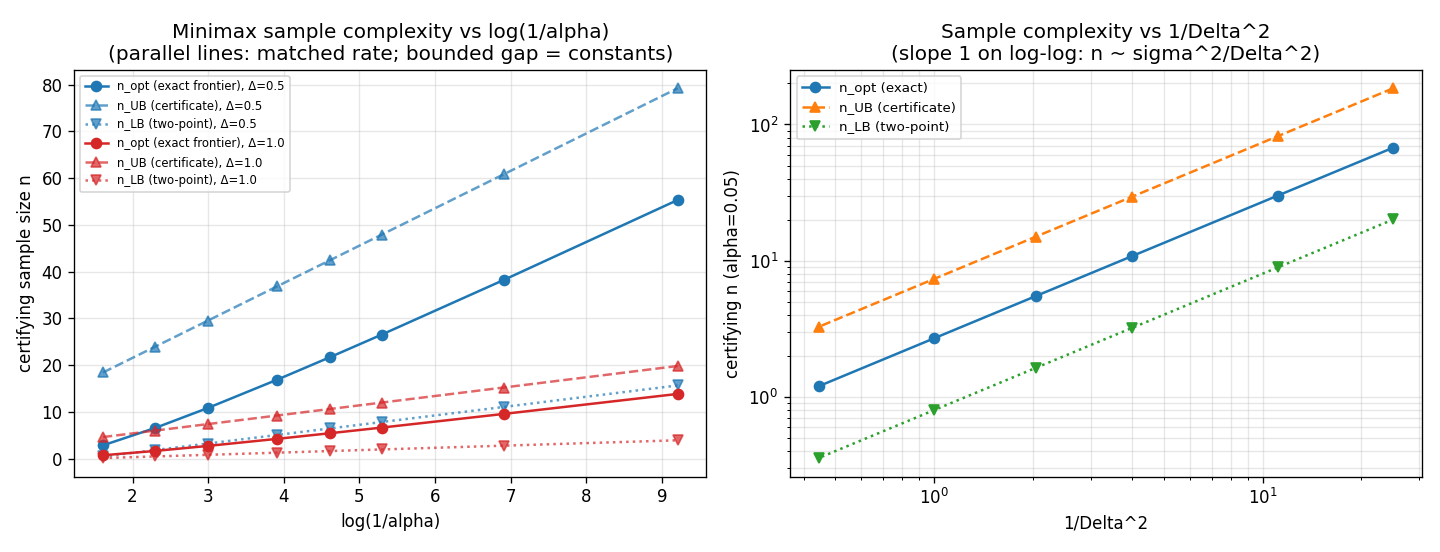
\includegraphics[width=0.92\linewidth]{theory_v2/fig_minimax_optimality.png}
\caption{Minimax order-optimality on the identifiable side (Theorem~\ref{thm:minimax-opt}).
Left: the exact certifying frontier $n_{\mathrm{opt}}$, the certificate upper bound
$n_{\mathrm{UB}}$, and the two-point lower bound $n_{\mathrm{LB}}$ are parallel and linear in
$\log(1/\alpha)$ (matched rate; the bounded vertical gaps are universal constants). Right: all
three lie on slope-$1$ log--log lines in $1/\Delta^2$, i.e.\ $n\asymp\sigma^2/\Delta^2$.}
\label{fig:minimax-opt}
\end{figure}
